\documentclass[tikz,border=10pt]{standalone}
\begin{document}
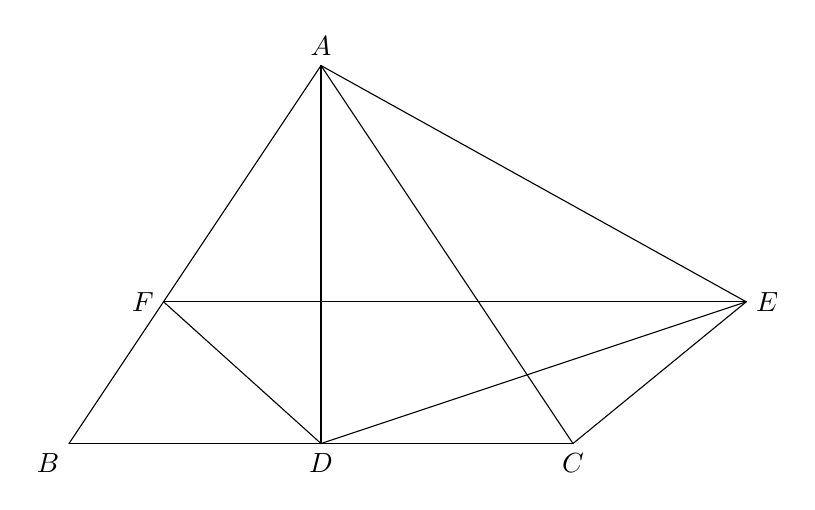
\begin{tikzpicture}[line cap=round,line join=round,scale=1]

\coordinate (B) at (0,0);
\coordinate (D) at (3.2,0);
\coordinate (C) at (6.4,0);
\coordinate (A) at (3.2,4.8);
\coordinate (F) at (1.2,1.8);
\coordinate (E) at (8.6,1.8);

\draw (B) -- (D) -- (C);
\draw (B) -- (A);
\draw (A) -- (D);
\draw (A) -- (C);
\draw (A) -- (E);
\draw (D) -- (E);
\draw (C) -- (E);
\draw (F) -- (D);
\draw (F) -- (E);

\node[above] at (A) {$A$};
\node[below left] at (B) {$B$};
\node[below] at (D) {$D$};
\node[below] at (C) {$C$};
\node[left] at (F) {$F$};
\node[right] at (E) {$E$};

\end{tikzpicture}
\end{document}
